\documentclass[../Notas.tex]{subfiles}
\graphicspath{{\subfix{../images/}}}

\begin{document}
\section{Noções de Análise Combinatória}
Dado um conjunto finito $S$, apresentaremos algumas maneiras de contar seus elementos, isto é, obter $|S|$. Desejamos fazer isto para calcular as probabilidades de eventos em espaços de probabilidade uniformes com espaço amostral finito já que, como vimos anteriormente, a probabilidade de um evento $A$ neste espaço nada mais é que $|A|/|\Omega|$.

\subsection{Amostras ordenadas}
Sejam $S = \{ s_1, \dots, s_n \}$ e $T = \{t_1, \dots, t_n\}$. Temos $|S| = m$ e $|T| = n$, de modo que $\Omega = S\times T = \{ (s,t) : s\in S, t\in T \}$ é tal que $|\Omega| = mn$. De maneira geral, se $S_1, \dots, S_n$ são tais que $|S_i| = m_i, 1\leq i\leq n$, então $\Omega = S_1\times S_2\times\cdots\times S_n = \{ (s_1, \dots, s_n) : s_i\in S_i, 1\leq i\leq n \}$ é tal que $|\Omega| = m_1\cdots m_n$. Note que se $m = m_1 = \cdots = m_n$, então $|\Omega| = m^n$.

\subsubsection{Amostragem com reposição}
Considere uma caixa com $m$ bolas numeradas de $1$ a $m$ em que retiramos uma bola, registramos seu número e a repomos na caixa. Repetimos esse procedimento $n$ vezes. Temos, então
\begin{align*}
    \Omega = \{ (x_1, \dots, x_n) : 1\leq x_i\leq n, 1\leq i\leq n \},
\end{align*}
sendo $x_i$ o número da $i$-ésima bola retirada, de modo que
\begin{align*}
    |\Omega| = m^n \ \text{(total de amostras de tamanho } n \text{\textbf{ com reposição})}.
\end{align*}

\begin{example}
Seja $\mathcal{E}$ o experimento que consiste em lançar $n$ vezes uma moeda honesta e observar o resultado. Qual a probabilidade de se obter pelo menos uma cara entre $n$ lançamentos? Ora, note que $\mathcal{E} \leftrightarrow$ extrair uma amostra de tamanho $n$, com reposição, de uma população com 2 elementos, $S = \{ c, \widehat{c} \}$. Temos
\begin{align*}
    \Omega = \{ (x_1, \dots, x_n) : x_i = c, \widehat{c}, i = 1, \dots, n \}.
\end{align*}
Daí, $|\Omega| = 2^n$ e tomamos $\mathcal{A} = \mathcal{P}(\Omega)$ e $P(\{\omega\}) = 1/2^n, \forall \omega\in\Omega$, de modo que $P(A) = |A|/2^n, \forall A\in\mathcal{A}$. Se $A = \{\text{obter pelo menos uma cara}\}\subset\Omega$, então $A^C = \{\text{não obter nenhuma cara nos } n \text{ lançamentos}\} = \{ (\widehat{c}, \dots, \widehat{c}) \}$. Logo, $P(A) = 1 - P(A^C) = 1 - 1/2^n$.
\end{example}

\subsubsection{Amostragem sem reposição (arranjos e permutações)}
Considere $S$ um conjunto com $m$ objetos distintos, $S = \{s_1, \dots, s_m\}$. Selecionamos um objeto de $S$ e não o repomos, repetindo esse processo $n \leq m$ vezes. Temos, então,
\begin{align*}
    \Omega = \{ (s_1, \dots, s_n) : s_i\in S, 1\leq i\leq n, s_i\neq s_j \forall i\neq j \}
\end{align*}
e, portanto, 
\begin{align*}
    |\Omega| = m(m-1)\cdots (m - n + 1) = \frac{m!}{(m-n)!} = A_{m,n}.
\end{align*}
Note que se $n=m$, então $A_{m,n} = A_{n,m} = P_m$ (permutação de $m$ elementos).

\begin{example}
Considere que temos 10 bolas numeradas de 1 a 10, $S = \{ 1, \dots, 10 \}$, e 3 caixas distintas. Suponha que queiramos escolher ao acaso 3 bolas, sem reposição, e colocar cada uma em uma das caixas. Temos
\begin{align*}
    \Omega = \{ (x_1, x_2, x_3) : x_i\in S, i=1,2,3, x_i\neq x_j, i\neq j \}.
\end{align*}
Note que, aqui, estamos considerando $(5,2,4)\neq (4,2,5)$ por exemplo, pois as caixas são distintas. Tomamos $\mathcal{A} = \mathcal{P}(\Omega)$ e $P(\{\omega\}) = 1/|\Omega|, \forall \omega\in\Omega$, com $|\Omega| = A_{10,3} = 10!/7! = 720$. Se tivéssemos $n$ bolas e $n$ caixas, então
\begin{align*}
    \Omega = \{ (x_1, \dots, x_n) : x_i\in S, i=1, \dots, n, x_i\neq x_j, i\neq j \},
\end{align*}
sendo $S = \{1, \dots, n\}$. Daí, temos $|\Omega| = n!$ e tomamos $\mathcal{A} = \mathcal{P}(\Omega)$ e $P(\{\omega\}) = 1/n!, \forall\omega\in\Omega$. Seja $A_{ij} = \{\text{bola i na caixa j}\}$, com $i , j\in S$ fixos. Note que $|A_{ij}| = (n-1)!$. Logo, $P(A_{ij}) = (n-1)!/n! = 1/n$ e, de modo geral, se $A_k = \{ \text{k bolas específicas em k caixas específicas} \}$, então $|A_k| = (n-k)!$ e $P(A_k) = (n-k)!/n! = 1/A_{n,k}$.
\end{example}

\subsection{Amostras desordenadas e sem reposição (combinações)}
Considere $S$ com $m$ objetos numerados distintos, $S = \{1, \dots, m\}$. Escolhemos, ao acaso, $r\leq m$ elementos de $S$, sem reposição e sem considerar a ordem de escolha. Temos
\begin{align*}
    \Omega = \{ (x_1, \dots, x_r) : x_i\in S, i=1,\dots, r, x_i < x_j, i<j \}.
\end{align*}
Daí, $|\Omega| = m!/(r!(m-r)!) = C_{m,r}$. De fato, se $|\Omega|\cdot P_r = A_{m,r}$, donde segue que $\Omega$ tem a forma acima. Denotamos também $C_{m,r} = \binom{m}{r}$.
\begin{example}
Sejam $S = \{ 1, 2, 3, 4 \}$, $r=3$. O número de amostras é $A_{4,3}/3! = 4 = C_{4,3}$.
\end{example}
\begin{example}
Suponha que há 75 professores no departamento de Matemática, sendo 25 titulares, 15 adjuntos e 35 assistentes. Queremos formar uma comissão de 6 membros, selecionados ao acaso. Seja $A = \{ \text{todos são assistentes} \}$. Temos
\begin{align*}
    \Omega = \{ (x_1, \dots, x_6) : x_i\in \{ 1, \dots, 75 \}, i=1,\dots, 6 \text{ e } x_i<x_j, i<j\}.
\end{align*}
Daí, $|\Omega| = \binom{75}{6}$ e, ademais, $A = \binom{35}{6}$, de modo que $P(A) = \binom{35}{6}/\binom{75}{6} \approx 1\%$.
\end{example}

\subsection{Permutações com elementos repetidos}
\paragraph{(a).} Considere um conjunto de $n$ objetos distintos, agrupados em $r$ espécies distintas: $n_1$ da espécie 1, $n_2$ da espécie 2,..., $n_r$ da espécie $r$, com $n_1 + \cdots + n_r = n$. A quantidade de permutações dos $n$ objetos é
\begin{align*}
    P_{n}^{n_1, \dots, n_r} &= \underbrace{\binom{n}{n_1}}_{\text{lugares 1ª espécie}}\binom{n-n_1}{n_2}\cdots\binom{n - (n_1 + n_2 + \cdots + n_{r-1})}{n_r} \\
    &= \frac{n!}{n_1!(n-n_1)!}\cdot\frac{(n-n_1)!}{n_2!(n-(n_1+n_2))!}\cdots\frac{(n-(n_1+\cdots+n_{r-1}))!}{n_r!(n-(n_1+\cdots+n_r))!} \\
    &= \frac{n!}{n_1!n_2!\cdots n_r!}.
\end{align*}
Denotamos também $\displaystyle{ P_n^{n_1, \dots, n_r} = \binom{n}{n_1, n_2, \dots, n_r} }$. Note que se $n_i = 1, i=1,\dots,r$, então $P_n^{n_1, \dots, n_r} = P_n^{1,\dots, 1} = P_n = n!$ e, se $r=2$, então
\begin{align*}
    \binom{n}{n_1, n_2} = \frac{n!}{n_1!n_2!} = \begin{cases}
        \frac{n!}{n_1!(n-n_1)!} &= \binom{n}{n_1} \\
        \frac{n!}{n_2!(n-n_2)!} &= \binom{n}{n_2} \\
    \end{cases}.
\end{align*}

\paragraph{(b).} Considere um conjunto com $n$ item distintos que deve ser dividido em $r$ grupos distintos de tamanhos $n_1, \dots, n_r$, com $n_1 + \cdots + n_r = r$. O total de divisões possíveis é $\displaystyle{ P_n^{n_1, \dots, n_r} = \binom{n}{n_1, n_2, \dots, n_r} }$. Note que tanto a expansão binomial quanto a multinomial usam desse raciocínio.

\subsection{Partições --- problema da urna}
\subsubsection{Urna simples}
Em uma urna, temos $n$ bolas: $n_A$ do tipo $A$ e $n_B$ do tipo $B$. Retira-se $m\leq n$ bolas ao acaso. Queremos calcular a probabilidade de $A_k = \{ \text{a amostra tem exatamente k bolas do tipo A} \}$. Note que $0\leq k\leq\min\{ n_A, m \}$ se não houver reposição e $0\leq k\leq m$ se houver reposição. Supondo resultados equiprováveis, temos $P(A_k) = |A_k|/|\Omega|$. Note que se $x_i$ são as bolas do tipo $A$ e $y_j$ são as bolas do tipo $B$, então
\begin{align*}
    \Omega = \{ x_1, \dots, x_{n_A}, y_1, \dots, y_{n_B} \}. 
\end{align*}
Ademais, $\Omega$ está em bijeção com $\{1, \dots, n_A, n_A + 1, \dots, n_A + n_B \}$, de modo que podemos pensar também $\Omega = \{ 1, \dots, n \}$.

\paragraph{Amostragem sem reposição.} Ao considerar $A_k$, queremos apenas a quantidade de bolas de cada tipo escolhidas, sem importar a ordem. Isso sugere que $P(A_k)$ fica inalterada se considerarmos ou não a ordem, e veremos que esse, de fato, é o caso. 

\begin{itemize}
    \item[(a1)] Considerando amostras não ordenadas, temos
    \begin{align*}
        \Omega = \{ \omega = (\omega_1, \dots, \omega_n) : \omega_i\in S, i = 1, \dots, m, \omega_i < \omega_j, i < j \},
    \end{align*}
    $\mathcal{A} = \mathcal{P}(\Omega)$ e $P(A) = |A|/|\Omega|, \forall A\in\mathcal{A}$. Note que $\displaystyle{|\Omega| = \binom{n}{m}}$ e, para todo $0\leq k\leq\min\{n_A,m\}$, temos $\displaystyle{|A_k| = \binom{n_A}{k}\binom{n_B}{m-k}}$. Daí, temos
    \begin{align*}
        P(A_k) = \frac{\binom{n_A}{k}\binom{n_B}{m-k}}{\binom{n}{m}} = \frac{\binom{n_A}{k}\binom{n-n_A}{m-k}}{\binom{n}{m}}, 0\leq k\leq\min\{n_A, m\},
    \end{align*}
    chamada de \textbf{probabilidade hipergeométrica}.
    
    \item[(a2)] Considerando amostras ordenadas, temos
    \begin{align*}
        \Omega = \{ \omega = (\omega_1, \dots, \omega_m) : \omega_i\in S_i, i=1, \dots, m \text{ e } \omega_i\neq\omega_j, i\neq j \}. 
    \end{align*}
    A $\sigma$-álgebra e a medida de probabilidade são as mesmas do caso acima. Agora, temos $|\Omega| = A_{n,m}$ e, para todo $0\leq k\leq\min\{n_A, m\}$, $\displaystyle{|A_k| = \binom{m}{k, m-k}A_{n_A, k}A_{n_b, m-k}}$. Daí,
    \begin{align*}
        P(A_k) = \frac{ \binom{m}{k}\frac{n_A!}{(n_A - k)!}\cdot\frac{n_B!}{(n_B - m + k)!} }{\frac{n!}{(n-m)!}} = \frac{ \binom{n_A}{k}\binom{n_B}{m-k} }{\binom{n}{m}}.
    \end{align*}
\end{itemize}

\paragraph{Amostragem com reposição.} Neste caso, temos
\begin{align*}
    \Omega = \{ \omega = (\omega_1, \dots, \omega_m) : \omega_i \in S, i = 1, \dots, m \},
\end{align*}
com $m\leq n$ e $\mathcal{A}$ e $P$ como acima. Note que $|\Omega| = n^m$ e, para todo $k\in\{0, \dots, m\}$, $\displaystyle{|A_k| = \binom{m}{k, m-k}n_A^kn_B^{m-k} }$ e $\displaystyle{P(A_k) = \binom{m}{k}\frac{n_A^kn_B^{m-k}}{n^m}, k = 0, \dots, m }$, chamada de \textbf{probabilidade binomial}. Note também que se considerarmos a retirada de uma bola do tipo $A$ como ``sucesso'', então $P(\text{sucesso}) = n_A/n := p$ e $P(\text{fracasso}) = 1 - n_A/n = 1 - p$. Devido à reposição, os resultados das retiradas são mutuamente independentes, de modo que $P(A_k) = \displaystyle{ P(\text{exatamente k sucessos}) = \binom{m}{k}p^k(1-p)^{m-k}, k=0, \dots, m }$.


\subsubsection{Urna geral}
Agora, consideremos que em uma urna há $n$ bolas, sendo $n_i$ do tipo $i$, com $i = 1, \dots, r$. Note que $n_1 + \cdots + n_r = n$. Retiramos $m\leq n$ bolas ao acaso, e estamos interessados em calcular a probabilidade de $A = A_{k_1, \dots, k_r} = \{ \text{conter } k_i \text{ bolas do tipo } i, i = 1, \dots, r \}$, com $k_1 + \cdots + k_r = m$. Note que $0\leq k_i\leq\min\{n_i, m\}, i=1, \dots, r$ se não houver reposição e $0\leq k_i\leq m, i=1, \dots, r$ caso contrário. Sem perda de generalidade, podemos descrever o conjunto de bolas como $S = \{1, \dots, n \}$.

\paragraph{Amostragem sem reposição.} Como no caso da urna simples, a ordem não importa e temos
\begin{align*}
    \Omega = \{ \omega = (\omega_1, \dots, \omega_m) : \omega_i\in S, i=1, \dots, m, \omega_i<\omega_j, i<j \},
\end{align*}
$|\Omega| = \displaystyle{\binom{n}{m}}$ e $|A| = \displaystyle{ \binom{n_1}{k_1}\binom{n_2}{k_2}\cdots\binom{n_r}{k_r} }$, logo 
\begin{align*}
P(A) = \displaystyle{ \binom{n_1}{k_1}\cdots\binom{n_r}{k_r}/\binom{n}{m}}.
\end{align*}
\paragraph{Amostragem com reposição.} Analogamente ao caso da urna simples, temos $|\Omega| = n^m$, $|A| = \displaystyle{ \binom{m}{k_1, \dots, k_r}n_1^{k_1}\cdots n_r^{k_r} }$, logo 
\begin{align*}
    P(A) = \binom{m}{k_1, \dots, k_r}\frac{n_1^{k_1}\cdots n_r^{k_r}}{n^m}, 0\leq k_i\leq m, i = 1, \dots, r,
\end{align*}
chamada \textbf{probabilidade multinomial}. Observe que, em cada retirada, $P(\text{retirar bola do tipo } i) = n_i/n := p_i$. A reposição implica independência entre os resultados de cada retirada, logo
\begin{align*}
    P(A) = \binom{m}{k_1, \dots, k_r}p_1^{k_1}\cdots p_r^{k_r}.
\end{align*}
\begin{example}
Em um lote de 100 peças, 20 são defeituosas e 80 estão em perfeitas condições. Escolhe-se, ao acaso e sem reposição, 10 peças. Estamos interessados em calcular a probabilidade de que exatamente metade das peças escolhidas seja defeituosa. Note que aqui temos um problema de urna simples, com $n_1 = 20$, $n_2 = 80$, $m = 10$ e $k = 5$. Daí, sendo $A_k = \{\text{a amostra contém 5 peças defeituosas e 5 peças perfeitas}\}$, temos que
\begin{align*}
P(A_k) = \frac{\binom{20}{5}\binom{80}{5}}{\binom{100}{10}}.
\end{align*}
\end{example}

\section{Variáveis aleatórias}
%\subsection{Variáveis aleatórias}
Comecemos considerando o seguinte exemplo motivador: temos o experimento ``lançar uma moeda 3 vezes''. A cada lançamento, podemos obter $c$ (cara) com probabilidade $p$ ou $\widehat{c}$ (coroa) com probabilidade $1-p$. Suponha que ganhamos R\$1,00 para cada cara obtida e perdemos o mesmo valor para cada coroa obtida.  Assim, ao final do experimento, poderemos ter $-3, -1, 1$ ou 3 reais (onde $-x$ reais indica prejuízo de $x$ reais). Estamos interessados em calcular a probabilidade de cada um desses resultados. Nosso espaço de probabilidade é $(\Omega, \mathcal{A}, P)$ com
\begin{align*}
    \Omega = \{ (c,c,c), (c,c,\widehat{c}), (c, \widehat{c}, c), (\widehat{c}, c, c), (c, \widehat{c}, \widehat{c}), (\widehat{c}, c, \widehat{c}), (\widehat{c}, \widehat{c}, c), (\widehat{c}, \widehat{c}, \widehat{c}) \},
\end{align*}
$\mathcal{A} = \mathcal{P}(\Omega)$ e nossa medida de probabilidade é dada por
\begin{align*}
    P(\{(c,c,c)\}) &= p^3, P(\{(c,c,\widehat{c})\}) = P(\{(c,\widehat{c},c)\}) = P(\{(\widehat{c},c,c)\}) = p^2(1-p), \\
    P(\{(c,\widehat{c},\widehat{c})\}) &= P(\{(\widehat{c},c,\widehat{c})\}) = P(\{(\widehat{c},\widehat{c},c)\}) = p(1-p)^2, P(\{(\widehat{c},\widehat{c},\widehat{c})\}) = (1-p)^3.
\end{align*}
Definamos $X:\Omega\to\mathbb{R}$ tal que $X(\omega) = $ quantia obtida pelo resultado $\omega, \forall\omega\in\Omega$. Assim, temos
\begin{align*}
    X((c,c,c)) &= 3, X((c,c,\widehat{c})) = X((c,\widehat{c},c)) = X((\widehat{c},c,c)) = 1, \\
    X((c,\widehat{c},\widehat{c})) &= X((\widehat{c},c,\widehat{c})) = X((\widehat{c},\widehat{c},c)) = -1, X((\widehat{c},\widehat{c},\widehat{c})) = -3,
\end{align*}
ou seja, $\Im(X) = \{-3,-1,1,3\}$. Observe que
\begin{align*}
    \{X=3\} &:= \{\omega\in\Omega : X(\omega) = 3\} = \{(c,c,c)\} \subset\Omega \therefore \{X=3\}\in\mathcal{A} \\
    \{X=1\} &:= \{\omega\in\Omega : X(\omega) = 1\} = \{(c,c,\widehat{c}), (c,\widehat{c},c), (\widehat{c}, c, c)\} \subset\Omega \therefore \{X=1\}\in\mathcal{A} \\
    \{X=-1\} &:= \{\omega\in\Omega : X(\omega) = -1\} = \{(c,\widehat{c},\widehat{c}), (\widehat{c},c,\widehat{c}), (\widehat{c}, \widehat{c}, c)\} \subset\Omega \therefore \{X=-1\}\in\mathcal{A} \\
    \{X=-3\} &:= \{\omega\in\Omega : X(\omega) = -3\} = \{(\widehat{c}, \widehat{c}, \widehat{c})\} \subset\Omega \therefore \{X=-3\}\in\mathcal{A} \\
    \{X=x\} &:= \{\omega\in\Omega : X(\omega) = x\} = \emptyset\in\mathcal{A}, \forall x\in\mathbb{R}\setminus\Im(X).
\end{align*}
Ademais, $\{X=-3\}\cup\{X=-1\}\cup\{X=1\}\cup\{X=3\} = \Omega\in\mathcal{A}$ e note que
\begin{align*}
    \{X\leq 1\} &:= \{\omega\in\Omega : X(\omega) \leq 1\} = \{X=-3\}\cup\{X=-1\}\cup\{X=1\} \in\mathcal{A} \\
    \{X\leq 0,5\} &:= \{\omega\in\Omega : X(\omega) \leq 0,5\} = \{X=-3\}\cup\{X=-1\} \in\mathcal{A}.
\end{align*}
De maneira geral, como $\Im(X)\subset\mathbb{Z}$, então temos
\begin{align*}
    \{ X\leq x \} = \{ \omega\in\Omega : X(\omega) \leq x \} = \bigcup_{i: x_i\leq[x]}\{X = x_i\}\in\mathcal{A}, \ x_i \text{ valor possível para }x,
\end{align*}
ou seja, $\{X\leq x\}$ é um evento para todo $x$ real. Assim, podemos calcular
\begin{align*}
    P(X=3) &= p^3, P(X=1) = 3p^2(1-p), P(X=-1) = 3p(1-p)^2, \\
    P(X=-3) &= (1-p)^3 \text{ e } P(X=x) = 0, \forall x\in\mathbb{R}\setminus\Im(X).
\end{align*}

\begin{definition}[Variável aleatória]
Uma variável aleatória $X$ em um espaço de probabilidade $(\Omega, \mathcal{A}, P)$ é uma função $X:\Omega\to\mathbb{R}$ tal que $\{X\leq x\} = \{ \omega\in\Omega : X(\omega)\leq x\}\in\mathcal{A}, \forall x\in\mathbb{R}$.
\end{definition}

\begin{remarks}
\begin{enumerate}[(a)]
    \item Note que
    \begin{align*}
        \{ X\leq x \} = X^{-1}((-\infty, x]) = \{ \omega\in\Omega : X(\omega) \in (-\infty, x] \}, \forall x\in\mathbb{R}.
    \end{align*}
    \item De modo geral, $X:\Omega\to\mathbb{R}$ é uma variável aleatória (v.a.) em $(\Omega, \mathcal{A}, P)$ se
    \begin{align*}
        X^{-1}(B) = \{ \omega\in\Omega : X(\omega) X(\omega)\in B \}\in\mathcal{A}, \forall B\in\mathcal{B}(\mathbb{R}).
    \end{align*}
    \item Dado um espaço de probabilidade $(\Omega, \mathcal{A}, P),$ se
    \begin{itemize}
        \item $\Omega$ é enumerável (caso discreto), então $\mathcal{A} = \mathcal{P}(\Omega)$ e toda função $X\Omega\to\mathbb{R}$ é uma v.a. (não será demonstrado).
        \item $\Omega\subset\mathbb{R}^n, n\geq 1$ é não enumerável, então $\mathcal{A} = \mathcal{B}^n(\mathbb{R})$. Nesse caso, nem toda função $X:\Omega\to\mathbb{R}$ é uma v.a., mas as exceções são raras.
    \end{itemize}
\end{enumerate}
Todas as funções que definirmos no contexto de v.a.'s serão de fato v.a.'s, e portanto não será necessário verificar pela definição.
\end{remarks}

\begin{examples}
\begin{enumerate}
    \item No experimento da motivação, $X$ é v.a.; de fato, vimos que $\{X\leq x\} \in\mathcal{A}, \forall x\in\mathbb{R}$.
    \item Suponha que um ponto é escolhido ao acaso no círculo unitário centrado na origem. Seja $Y$ a distância desse ponto à origem. Temos
    \begin{align*}
        \Omega = \{ (x,y)\in\mathbb{R}^2 : x^2 + y^2 \leq 1 \}, \mathcal{A} = \mathcal{B}^2(\Omega)
    \end{align*}
    e, $\forall A\in\mathcal{A}$, $\displaystyle{ P(A) = \iint_A \frac{1}{\pi}dxdy }$. Daí, como $Y:\Omega\to\mathbb{R}$ é dada por $Y(\omega) = Y((x,y)) = \sqrt{x^2 + y^2}$, temos que dado $z\in\mathbb{R}$,
    \begin{align*}
        \{ Y\leq z \} = \{ (x,y)\in\Omega : \sqrt{x^2 + y^2} \leq z \} = \begin{cases}
        \emptyset, z < 0, \\
        \{ (x,y) : \sqrt{x^2 + y^2} \leq z \}, 0\leq z < 1, \\
        \Omega, z\geq 1
        \end{cases},
    \end{align*}
    ou seja, $\{Y\leq z\}\in\mathcal{A}, \forall z\in\mathbb{R}$, de modo que $Y$ é v.a. em $(\Omega, \mathcal{A}, P)$.
\end{enumerate}
\end{examples}

\begin{definition}
Seja $X$ v.a. em $(\Omega, \mathcal{A}, P)$.
\begin{enumerate}[(i)]
    \item $X$ é discreta se $\Im(X)\subset\mathbb{R}$ é finita ou enumerável;
    \item $X$ é contínua se $P(X=x) = 0, \forall x\in\mathbb{R}$.
\end{enumerate}
\end{definition}
Note que se $X$ é v.a. discreta com imagem enumerável, digamos $\Im(X) = \{ x_1, x_2, \dots \}$, então
\begin{enumerate}[(a)]
    \item $P(X = x_i) > 0, i = 1, 2, \dots$
    \item $P(X = x_i) = 0, x\neq x_i, i = 1, 2, \dots$
    \item $\displaystyle{ \bigcup_{i=1}^{\infty} \{X = x_i\} = \Omega}$
    \item $\displaystyle{ \sum_{i=1}^{\infty}P(X = x_i) = 1 }$
\end{enumerate}

\begin{example}
No Exemplo 1 anterior, $X$ é v.a. discreta e, no Exemplo 2, $Y$ é v.a. contínua pois $P(Y=z) = \{ (x,y)\in\Omega : x^2 + y^2 = z^2 \} = 0, \forall z\in\mathbb{R}$.
\end{example}

Concentraremos o nosso estudo primeiro nas v.a.'s discretas e, mais à frente, nas contínuas.

\subsection{Variáveis aleatórias discretas}
No estudo das v.a.'s, tanto discretas quanto contínuas, utilizamos de funções que determinam o ``comportamento'' da referida v.a.; no caso de v.a.'s discretas, temos a \textbf{função de probabilidade (f.p.)} e a \textbf{função de distribuição (f.d.)}. Começamos pela função de probabilidade.
\begin{definition}
Seja $X$ v.a. discreta em $(\Omega, \mathcal{A}, P)$. A \textbf{função de probabilidade de } $X$ é a função $p_X:\mathbb{R}\to [0,1]$ dada por
\begin{align*}
    p_X(x) = P(X=x), \forall x\in\mathbb{R}.
\end{align*}
\end{definition}
A função de probabilidade associa, a cada número real, a probabilidade de $X$ assumir tal valor.
\begin{remark}
Se $x\in\mathbb{R}$ é tal que $p_X(x) > 0$, dizemos que $x$ é um \textbf{valor possível} de $X$. Além disso, note que se $X$ é discreta então existe $\{ x_1, x_2, \dots \}\subset\mathbb{R}$ finito ou enumerável tal que $p_X(x_i) > 0, i=1,2,\dots$ e $p_X(x) = 0, x\notin\{x_1, x_2, \dots\}$. Como os eventos $\{X = x_i\}, i=1, 2, \dots$ são disjuntos e $\displaystyle{ \bigcup_{i=1}^{\infty} \{X=x_i\} = \Omega}$ (ou seja, esses eventos formam uma partição de $\Omega$), segue que $\displaystyle{ \sum_{i=1}^{\infty}p_X(x_i) = 1 }$.
\end{remark}

\begin{example}
No exemplo motivador, temos $P(\text{cara}) = p = 1/2$. A função de probabilidade de $X$ é dada por $p_X(-3) = P(X=-3) = 1/8$, $p_X(-1) = p_X(1) = 3/8$, $p_X(3) = 1/8$ e $p_X(x) = 0, \forall x\in\mathbb{R}\setminus\{0,1\}$.
\end{example}

\begin{example}
Dados $(\Omega, \mathcal{A}, P)$ espaço de probabilidade e $c\in\mathbb{R}$ constante, defina $X:\Omega\to\mathbb{R}$ tal que $X(\omega) = c, \forall\omega\in\Omega$. Daí, dado $x\in\mathbb{R}$,
\begin{align*}
    \{X\leq x\} = \begin{cases}
    \emptyset, x < c \\
    \Omega, x\geq c
    \end{cases}\in\mathcal{A},
\end{align*}
ou seja, $X$ é v.a. Como $P(X=c) = P(\Omega) = 1$ e $P(X=x) = 0, x\neq c$, temos que $X$ é v.a. discreta com apenas um valor possível, $c$.
\end{example}

\begin{example}
Dados $(\Omega, \mathcal{A}, P)$ espaço de probabilidade e $A\in\mathcal{A}$, defina $X:\Omega\to\mathbb{R}$ tal que
\begin{align*}
    X(\omega) = \begin{cases}
    1, \omega\in A \\
    0, \omega\notin A
    \end{cases}.
\end{align*}
Daí, dado $x\in\mathbb{R}$ temos
\begin{align*}
    \{X\leq x\} = \begin{cases}
    \emptyset, x < 0 \\
    A^C, 0\leq x < 1 \\
    \Omega, x\geq 1
    \end{cases}\in\mathcal{A},
\end{align*}
logo $X$ é v.a. com dois valores possíveis, 0 e 1, chamada de \textbf{v.a. indicadora de A}, usualmente denotada por $I_A$ ou $1_A$. Se considerarmos $P(A) = p$, temos
\begin{align*}
    p_X(x) = \begin{cases}
    p, x = 1 \\
    1 - p, x = 0 \\
    0, x\in\mathbb{R}\setminus\{0,1\}
    \end{cases} \text{ (função de probabilidade \textbf{Bernoulli} de parâmetro } p)
\end{align*}
Reciprocamente, se $X$ é uma v.a. discreta definida em $(\Omega, \mathcal{A}, P)$ com conjunto de valores possíveis $\{0,1\}$, então $X$ é v.a. indicadora. De fato, denotando $P(X=1) = P(A) = p$, a função de probabilidade de $X$ é dada por
\begin{align*}
    p_X(x) = \begin{cases}
    p, x = 1 \\
    1 - p, x = 0 \\
    0, x\in\mathbb{R}\setminus\{0,1\}
    \end{cases}.
\end{align*}
Logo, $X = 1_A$ sendo $A = \{ \omega\in\Omega : X(\omega) = 1 \}$.
\end{example}

\begin{proposition}
Seja $X$ v.a. discreta em $(\Omega, \mathcal{A}, P)$. A função de probabilidade de $X$, $p_X$, é tal que
\begin{itemize}
    \item[(P1)] $p_X(x) \geq 0, \forall x\in\mathbb{R}$;
    \item[(P2)] $\{ x\in\mathbb{R} : p_X(x) \neq 0 \} = \{ x_1, x_2, \dots \}\subset\mathbb{R}$ é finito ou infinito enumerável;
    \item[(P3)] $\displaystyle{ \sum_{i=1}^{\infty}p_X(x_i) = 1. }$
\end{itemize}
\end{proposition}
\begin{proof}
Os três itens seguem da definição de v.a. discreta e das propriedades da medida de probabilidade.
\end{proof}

\begin{definition}[Função de probabilidade]
Dizemos que $p:\mathbb{R}\to\mathbb{R}$ é uma \textbf{função de probabilidade} se satisfaz (P1), (P2) e (P3).
\end{definition}

\begin{proposition}
Se $p:\mathbb{R}\to\mathbb{R}$ é uma função de probabilidade, então existe um espaço de probabilidade $(\Omega, \mathcal{A}, P)$ e uma v.a. $X$ definida neste espaço tal que $p=p_X$.
\end{proposition}

\begin{proof}
Por hipótese, $p$ é f.p., logo $\{ x\in\mathbb{R} : p_X(x) \neq 0 \} = \{ x\in\mathbb{R} : p_X(x) > 0 \} = \{ x_1, x_2, \dots \}\subset\mathbb{R}$ é finito ou enumerável. Tomemos $\Omega = \{ x_1, x_2, \dots \}$, $\mathcal{A} = \mathcal{P}(\Omega)$ e $P:\mathcal{A}\to\mathbb{R}$ dada por
\begin{align*}
    P(\{x_i\}) = p(x_i), i = 1, 2, \dots
\end{align*}
e, dado $A\in\mathcal{A}$,
\begin{align*}
    P(A) = \sum_{i : x_i\in A} p(x_i).
\end{align*}
De (P1) e (P3), segue que $P$ é medida de probabilidade em $(\Omega, \mathcal{A})$. Definamos $X:\Omega\to\mathbb{R}$ tal que
\begin{align*}
    X(\omega) = \omega \Longleftrightarrow X(x_i) = x_i, i=1,2,\dots
\end{align*}
Então $X$ é v.a. discreta com valores possíveis $x_1, x_2, \dots$ e f.p.
\begin{align*}
    p_X(x_i) = P(X=x_i) = P(\{ \omega\in\Omega : X(x_i) = x_i \}) = P(\{x_i\}) = p(x_i), i = 1,2, \dots
\end{align*}
\end{proof}

\subsection{Exemplos clássicos de v.a.'s discretas}
\begin{example}[Uniforme discreta]
Sejam $\mathcal{E}$ um experimento com $n$ resultados possíveis e equiprováveis, $\Omega = \{ \omega_1, \dots, \omega_n \}$, $\mathcal{A} = \mathcal{P}(\Omega)$ e $P:\mathcal{A}\to\mathbb{R}$ dada por $P(A) = |A|/|\Omega|$. Seja $X:\Omega\to\mathbb{R}$ dada por $X(\omega_i) = x_i, i = 1, 2, \dots, n$. $X$ é v.a. com valores possíveis $\{x_1, \dots, x_n\}$, e temos
\begin{align*}
    p_X(x) = P(X=x) = \begin{cases}
    1/n, x\in\{x_1, \dots, x_n\} \\
    0, \text{ c.c.}
    \end{cases}.
\end{align*}
\end{example}

\begin{example}[Binomial de parâmetros $n$ e $p$, $X\sim B(n,p)$]
Sejam $\mathcal{E}$ um experimento, $(\Omega, \mathcal{A}, P)$ espaço de probabilidade e $A$ um evento associado a $\mathcal{E}$ tal que $P(A) = p$ (sucesso) e, consequentemente, $P(A^C) = 1 - p$ (fracasso), com $0 < p < 1$. Suponha que são realizadas $n\geq 1$ repetições \textbf{independentes} de $\mathcal{E}$ (provas ou ensaios de Bernoulli), e seja $X$ o número de ocorrências de $A$ (sucessos) nas $n$ repetições. Temos $X$ v.a. com conjunto de valores possíveis $\{0, 1, \dots, n\}$, donde
\begin{align*}
    p_X(k) = P(X=k) = \begin{cases}
    \binom{n}{k}p^k(1-p)^{n-k}, k = 0, 1, \dots, n \\
    0, \text{ c.c.}
    \end{cases}.
\end{align*}
Note que a função $p:= p_X$ define uma função de probabilidade.
\begin{proof}
\begin{itemize}
    \item[(P1)] $p_X(x) = \binom{n}{x}p^x(1-p)^{n-x} > 0$ para $x\in\{0, 1, \dots, n\}$ e $p_X(x) = 0$ para $x\in\mathbb{R}\setminus\{0, 1, \dots, n\}$.
    \item[(P2)] $\{ x\in\mathbb{R} : p_X(x)\neq 0 \} = \{ 0, 1, \dots, n \}$ é finito.
    \item[(P3)] $\displaystyle{ \sum_i p_X(x_i) = \sum_{k=0}^{n} p_X(k) = \sum_{k=0}^{n}\binom{n}{k}p^k(1-p)^{n-k} = (p + 1-p)^n = 1 }$.
\end{itemize}
\end{proof}
Se $n=1$, $X$ é v.a. \textbf{de Bernoulli} de parâmetro $p$:
\begin{align*}
    p_X(k) = \begin{cases}
    p, k = 1 \\
    1 - p, k = 0 \\
    0, \text{ c.c.}
    \end{cases}
\end{align*}
\end{example}

\begin{example}[Geométrica de parâmetro $p$, $X\sim \text{Geom}(p)$]
Sejam $\mathcal{E}$ um experimento, $(\Omega, \mathcal{A}, P)$ espaço de probabilidade e $A$ um evento associado a $\mathcal{E}$ tal que $P(A) = p$ (sucesso) e $P(A^C) = 1 - p$ (fracasso), com $ 0 < p < 1$. Repetimos $\mathcal{E}$ até que $A$ ocorra pela 1ª vez. Temos $X$ v.a. com conjunto de valores possíveis $\{ 1, 2, \dots,  \}$. Note que $\{ X = k \} = \{ A^C\text{ ocorre nas primeiras } k-1 \text{ repetições e } A \text{ ocorre na k-ésima} \}$. Daí,
\begin{align*}
    p_X(k) = P(X=k) = \begin{cases}
    p(1-p)^{k-1}, k = 1, 2, \dots \\
    0, \text{ c.c.}
    \end{cases}
\end{align*}
Note que a função $p:= p_X:\mathbb{R}\to\mathbb{R}$ define uma função de probabilidade.
\begin{proof}
\begin{itemize}
    \item[(P1)] $p_X(x) = p(1-p)^{x-1} > 0$ se $x\in\{1, 2, \dots\}$ e $p_X(x) = 0$ se $x\in\mathbb{R}\setminus\{1, 2, \dots\}$.
    \item[(P2)] $\{ x\in\mathbb{R} : p_X(x)\neq 0 \} = \{ 1, 2, \dots \}$ é enumerável.
    \item[(P3)] $\displaystyle{ \sum_i p_X(x_i) = \sum_{k=1}^{\infty}p(1-p)^{k-1} = p\frac{1}{p-1} = 1.}$
\end{itemize}
\end{proof}
Podemos também representar a f.p. da v.a. geométrica de parâmetros $n$ e $p$ por (vide Exercício 2b, Lista 3)
\begin{align*}
    p_X(k) = \begin{cases}
    p(1-p)^k, k = 0, 1, \dots \\
    0, \text{ c.c.}
    \end{cases}
\end{align*}
\end{example}

\begin{example}[Binomial negativa de parâmetros $r$ e $p$, $X\sim BN(r,p)$]
Estamos na mesma situação da v.a. geométrica, mas agora $X$ é o número de repetições necessárias para que $A$ ocorra exatamente $r$ vezes. $X$ é uma v.a. com conjunto de valores possíveis $\{ r, r+1, \dots \}$. Note que $\{ X=k \} = \{ A \text{ ocorre na k-ésima repetição e em exatamente } r-1 \text{ vezes nas } k-1 \text{ repetições anteriores} \}$. Daí,
\begin{align*}
    p_X(k) = P(X=k) =\begin{cases}
    \binom{k-1}{r-1}p^r(1-p)^{k-r}, k = r, r+1, \dots \\
    0, \text{ c.c.}
    \end{cases}.
\end{align*}
Note que se $r=1$, $X\sim\text{Geo}(p)$. Ademais, se definirmos $\displaystyle{ \binom{-r}{0} = 1 }$ e $\displaystyle{ \binom{-r}{m} = (-1)^m\cdot\frac{(r+1)\cdots (r+m-1)}{m!}, m\geq 1 }$, temos $\displaystyle{ \binom{k-1}{r-1} = (-1)^{k-r}\binom{-r}{k-r}, k = r, r+1, \dots }$. Daí, podemos reescrever $p_X$ como
\begin{align*}
    p_X(k) = \begin{cases}
    \binom{-r}{k-r}(-1)^{k-r}p^r(1-p)^{k-r}, k = r, r+1, \dots \\
    0, \text{ c.c.}
    \end{cases}.
\end{align*}
Note também que $p:=p_X:\mathbb{R}\to\mathbb{R}$ dada acima (usaremos a primeira forma por simplicidade) é função de probabilidade.
\begin{proof}
\begin{itemize}
    \item[(P1)] $p_X(x) = \displaystyle{ \binom{k-1}{r-1}p^r(1-p)^{k-r} > 0 }$ se $x\in\{r, r+1, \dots\}$ e $p_X(x) = 0$ se $x\in\mathbb{R}\setminus\{r, r+1, \dots\}$.
    \item[(P2)] $\{ x\in\mathbb{R} : p_X(x) \neq 0 \} = \{r, r+1, \dots\}$ é enumerável.
    \item[(P3)] Temos
    \begin{align*}
        (1-t)^{-r} = \sum_{j=0}^{\infty}\underbrace{\binom{-r}{j}(-1)^j}_{\binom{j+r-1}{r-1}}t^j, |t| < 1.
    \end{align*}
    Logo, 
    \begin{align*}
        \sum_i p_X(x_i) = \sum_{k=r}^{\infty}\binom{k-1}{r-1}p^r(1-p)^{k-r} &= p^r\sum_{j=0}^{\infty}\binom{j+r-1}{r-1}(1-p)^j \\
        &= p^r\sum_{j=0}^{\infty}\binom{-r}{j}(-1)^j(1-p)^j \\
        &= p^r\frac{1}{p^r} = 1.
    \end{align*}
\end{itemize}
\end{proof}
Por fim, a f.p. da v.a. binomial negativa de parâmetros $r$ e $p$ pode ser reescrita como (vide Exercício 2c, Lista 3)
\begin{align*}
    p_X(k) = \begin{cases}
    \binom{r+k-1}{r-1}p^r(1-p)^{k}, k = 0, 1, \dots \\
    0, \text{ c.c.}
    \end{cases}
\end{align*}
\end{example}

\begin{example}[Hipergeométrica de parâmetros $N, r$ e $n$, $X\sim\text{Hgeo}(N,r,n)$]
Considere um conjunto com $N$ objetos, $r$ do tipo 1 e $N-r$ do tipo 2. Uma amostra de tamanho $n\leq r$ é selecionada, sem reposição. Seja $X$ o número de objetos do tipo 1 na amostra. Temos $X$ v.a. com conjunto de valores possíveis $\{ 0, 1, \dots, n \}$. Note que $\{ X=k \} = \{ \text{a amostra tem exatamente k objetos do tipo 1} \}$. Daí, 
\begin{align*}
    p_X(k) = \begin{cases}
    \frac{ \binom{r}{k}\binom{N-r}{n-k} }{\binom{N}{n}}, k = 0, 1, \dots, n \\
    0, \text{ c.c.}
    \end{cases}.
\end{align*}
Note que $p:=p_X:\mathbb{R}\to\mathbb{R}$ é, de fato, uma função de probabilidade.
\begin{proof}
\begin{itemize}
    \item[(P1)] $p_X(x) = \binom{r}{x}\binom{N-r}{n-x}/\binom{N}{n} > 0$ se $x\in\{ 0,1,\dots, n \}$ e $p_X(x) = 0$ se $x\in\mathbb{R}\setminus\{ 0,1,\dots, n \}$.
    \item[(P2)] $\{ x\in\mathbb{R} : p_X(x)\neq 0 \} = \{0, 1, \dots, n\}$ é finito.
    \item[(P3)] $\displaystyle{ \sum_i p_X(x_i) = \sum_{k=0}^{n}\frac{\binom{r}{k}\binom{N-r}{n-k}}{\binom{N}{n}} \stackrel{*}{=} \binom{N}{n}/\binom{N}{n} = 1,}$ onde em $*$ usamos a \textbf{identidade de Vandermonde}:
    \begin{align*}
        \binom{a+b}{n} = \sum_{k=0}^{n}\binom{a}{k}\binom{b}{n-k}, n\leq\min\{a,b\} \text{ e } a,b,\in\mathbb{N}.
    \end{align*}
\end{itemize}
\end{proof}
\end{example}

\begin{example}[Poisson com parâmetro $\lambda > 0$, $X\sim \text{Poisson}(\lambda)$]
Considere $n$ ensaios de Bernoulli com probabilidade de sucesso $p_n = \lambda/n, \lambda\in\mathbb{R}_{>0}$ fixo. Para cada $n\geq 1$, seja $X_n$ o número de sucessos nas $n$ provas. Daí, para cada $n$, temos $X_n\sim B(n, p_n)$, ou seja,
\begin{align*}
    P(X_n=k) = \begin{cases}
    \binom{n}{k}p_n^k(1-p_n)^{n-k}, k = 0, 1, \dots, n \\
    0, \text{ c.c.}
    \end{cases}.
\end{align*}
Note que para cada $k\in\{0,1,\dots, n\}$, temos
\begin{align*}
    P(X_n = k) &= \frac{n(n-1)\cdots (n-k+1)}{k!}\left(\frac{\lambda}{n}\right)^k\left(1-\frac{\lambda}{n}\right)^{n-k} \\
    &= \frac{\lambda^k}{k!}\cdot\frac{n(n-1)\cdots (n-k+1)}{n^k}\left(1-\frac{\lambda}{n}\right)^{-k}\left(1-\frac{\lambda}{n}\right)^n\xrightarrow{n\to\infty}e^{-\lambda}\frac{\lambda^k}{k!},
\end{align*}
de modo que
\begin{align*}
    p_X(k) = \begin{cases}
    e^{-\lambda}\lambda^k/k!, k = 0, 1, \dots \\
    0, \text{ c.c.}
    \end{cases}.
\end{align*}
Temos que $p:=p_X:\mathbb{R}\to\mathbb{R}$ define uma função de probabilidade.
\begin{proof}
\begin{itemize}
    \item[(P1)] $p(x) = e^{-\lambda}\lambda^k/k! > 0$ se $x\in\{0, 1, \dots\}$ e $p(x) = 0$ se $x\in\mathbb{R}\setminus\{0, 1, \dots\}$.
    \item[(P2)] $\{ x\in\mathbb{R} : p(x) \neq 0 \} = \{ 0, 1, \dots \}$ é enumerável.
    \item[(P3)] $\displaystyle{ \sum_i p(x_i) = \sum_{k=0}^{\infty}e^{-\lambda}\frac{\lambda^k}{k!} = e^{-\lambda}e^{\lambda} = 1}.$
\end{itemize}
\end{proof}
\end{example}

\begin{example}[Zipf ou zeta]
Colocamos este último exemplo de curiosidade. Uma v.a. $X$ tem distribuição zeta (ou Zipf) se sua f.p. é dada por
\begin{align*}
    p_X(k) = \begin{cases}
    \frac{C}{k^{\alpha + 1}}, k = 1, 2, \dots \\
    0, \text{ c.c.}
    \end{cases}, \alpha\in\mathbb{R}_{>0},
\end{align*}
onde
\begin{align*}
    C = \left[ \sum_{k=1}^{\infty}\left(\frac{1}{k}\right)^{\alpha + 1} \right]^{-1}.
\end{align*}
O nome de distribuição zeta vem do fato de que a função
\begin{align*}
    \zeta(s) = \sum_{n=1}^{\infty}\frac{1}{n^s}, s>1
\end{align*}
recebe o nome de \textbf{função zeta de Riemann}. Essa distribuição foi usada por um economista italiano, V. Pareto, para descrever a distribuição dos rendimentos das famílias de um dado país, mas foi G. K. Zipf(!) que aplicou a distribuição zeta em vários problemas de diferentes áreas, popularizando-a.
\end{example}

Tratada a f.p., passemos à função de distribuição. Agora, estamos interessados em calcular $P(X\in A) = P(\omega\in\Omega : X(\omega)\in A), \forall A\subset\mathbb{R}$. Consideraremos $X$ uma v.a. discreta definida em $(\Omega, \mathcal{A}, P)$ com f.p. $p_X$ e conjunto de valores possíveis $\{ x_1, x_2, \dots \}$ (finito ou enumerável). Note que dado $\mathcal{B}(\mathbb{R}) \ni A\subset\mathbb{R}$, $\{X\in A\}$ é um evento (pois $X$ é v.a.), de modo que faz sentido calcular $P(X\in A)$. Temos que
\begin{align*}
    P(X\in A) = P\left( \bigcup_{i : x_i\in A}\{ \omega\in\Omega : X(\omega) = x_i \} \right) &= \sum_{i : x_i\in A}P\left( \{ \omega\in\Omega : X(\omega) = x_i \} \right) \\
    &= \sum_{i : x_i\in A}P(X=x_i) \\
    &= \sum_{i : x_i\in A}p_X(x_i),
\end{align*}
ou seja,
\begin{align*}
    P(X\in A) = \sum_{i : x_i\in A} p_X(x_i).
\end{align*}
Portanto, vemos que a f.p. determina completamente a probabilidade $P(X\in A), \forall A\in\mathcal{B}(\mathbb{R})$.

\begin{definition}[Função de distribuição]
Se $X$ é uma v.a. definida em $(\Omega, \mathcal{A}, P)$, então $F_X:\mathbb{R}\to\mathbb{R}$ dada por
\begin{align*}
    F_X(x) = P(X\leq x) = P(X\in (-\infty, x]) = P(\omega\in\Omega : X(\omega)\leq x), \forall x\in\mathbb{R}
\end{align*}
é chamada \textbf{função de distribuição} de $X$.
\end{definition}
O exposto acima sugere que a f.p. determina por completo a f.d. de um v.a. $X$ qualquer. De fato, esse é o caso, e há, na verdade, uma relação biunívoca entre ambas, como mostra a seguinte proposição.
\begin{proposition}
Seja $X$ v.a. discreta definida em $(\Omega, \mathcal{A}, P)$ com conjunto de valores possíveis $\{ x_1, x_2, \dots \}$.
\begin{enumerate}[(a)]
    \item Se $X$ tem f.p. $p_X$, então $F_X$ é dada por
    \begin{align*}
        F_X(x) = P(X\leq x) = \sum_{i: x_i\leq x}p_X(x_i), \forall x\in\mathbb{R}.
    \end{align*}
    \item Suponha $x_1\leq x_2\leq\cdots$. Se $X$ tem f.d. $F_X$, então sua f.p. $p_X$ é dada por
    \begin{align*}
        p_X(x_i) = P(X=x_i) = F_X(x_i) - F_X(x_{i-1}), i = 1, 2, \dots
    \end{align*}
\end{enumerate}
\end{proposition}

\begin{proof}
\begin{enumerate}[(a)]
    \item Dado $x\in\mathbb{R}$, temos
    \begin{align*}
        F_X(x) = P(X\leq x) = P(X\in [-\infty, x]) = \sum_{i : x_i\leq x}P(X=x_i) = \sum_{i : x_i\leq x}p_X(x_i).
    \end{align*}
    \item Note que $\{ X\leq x_i \} = \{ X = x_i \} \sqcup \{ X < x_i \}$, donde
    \begin{align*}
        p_X(x_i) = P(X =x_i) &= P(X\leq x_i) - P(X<x_i) \\
        &= P(X\leq x_i) - P(X\leq x_{i-1}) \\
        &= F_X(x_i) - F_X(x_{i-1}), i = 1, 2, \dots
    \end{align*}
    em que a penúltima igualdade se deve ao fato de que $x_1\leq x_2\leq \cdots$.
\end{enumerate}
\end{proof}
Como mencionamos, essa proposição nos diz que há uma correspondência $F_X\leftrightarrow p_X$. Por causa disso, chamamos de \textbf{distribuição de probabilidade} de $X$ tanto $F_X$ quanto $p_X$. Também segue da proposição que se $X$ é v.a. discreta com conjunto de valores possíveis $\{x_1, x_2, \dots \}$ (como na proposição, podemos supor $x_1\leq x_2\leq\cdots$ sem perda de generalidade), então a f.d. $F_X$ é do tipo escada, com saltos em $x_1, x_2, \dots;$ o tamanho do salto em $x_i$ é $F_X(x_i) - F_X(x_{i-1}) = P(X=x_i)$. A soma dos saltos é 1, isto é, $\displaystyle{ \sum_{i\geq 1} \underbrace{F_X(x_i) - F_X(x_{i-1})}_{P(X=x_i)} = 1.}$ 

\begin{example}
Considere dois lançamentos independentes de uma moeda honesta. Seja $X$ o número de caras obtidas nos dois lançamentos. Temos $0, 1$ e $2$ como valores possíveis de $X$. A f.p. de $X$, $p_X$, é dada por
\begin{align*}
    p_X(0) = \frac{1}{2}\cdot\frac{1}{2} = \frac{1}{4}, \ p_X(1) = \frac{1}{4} + \frac{1}{4} = \frac{1}{2}, \ p_X(2) = \frac{1}{2}\cdot\frac{1}{2} = \frac{1}{4} \ \text{ e } \ p_X(x) = 0, x\in\mathbb{R}\setminus\{0, 1, 2\}.
\end{align*}
A f.d. de $X$, $F_X$, é dada por
\begin{align*}
    F_X(x) &= P(X\leq x) = P(\emptyset) = 0, x < 0 \\
    F_X(x) &= P(X\leq x) = P(X=0) = 1/4, 0\leq x < 1 \\
    F_X(x) &= P(X\leq x) = P(X=0) + P(X=1) = 3/4, 1\leq x < 2 \\
    F_X(x) &= P(X\leq x) = P(X=0) + P(X=1) + P(X-2) = 1, x\geq 2,
\end{align*}
ou seja, 
\begin{align*}
    F_X(x) = \begin{cases}
    0, x<0 \\
    1/4, 0\leq x < 1 \\
    3/4, 1\leq x < 2 \\
    1, x\geq 2
    \end{cases}
\end{align*}
\begin{figure}[H]
    \centering
    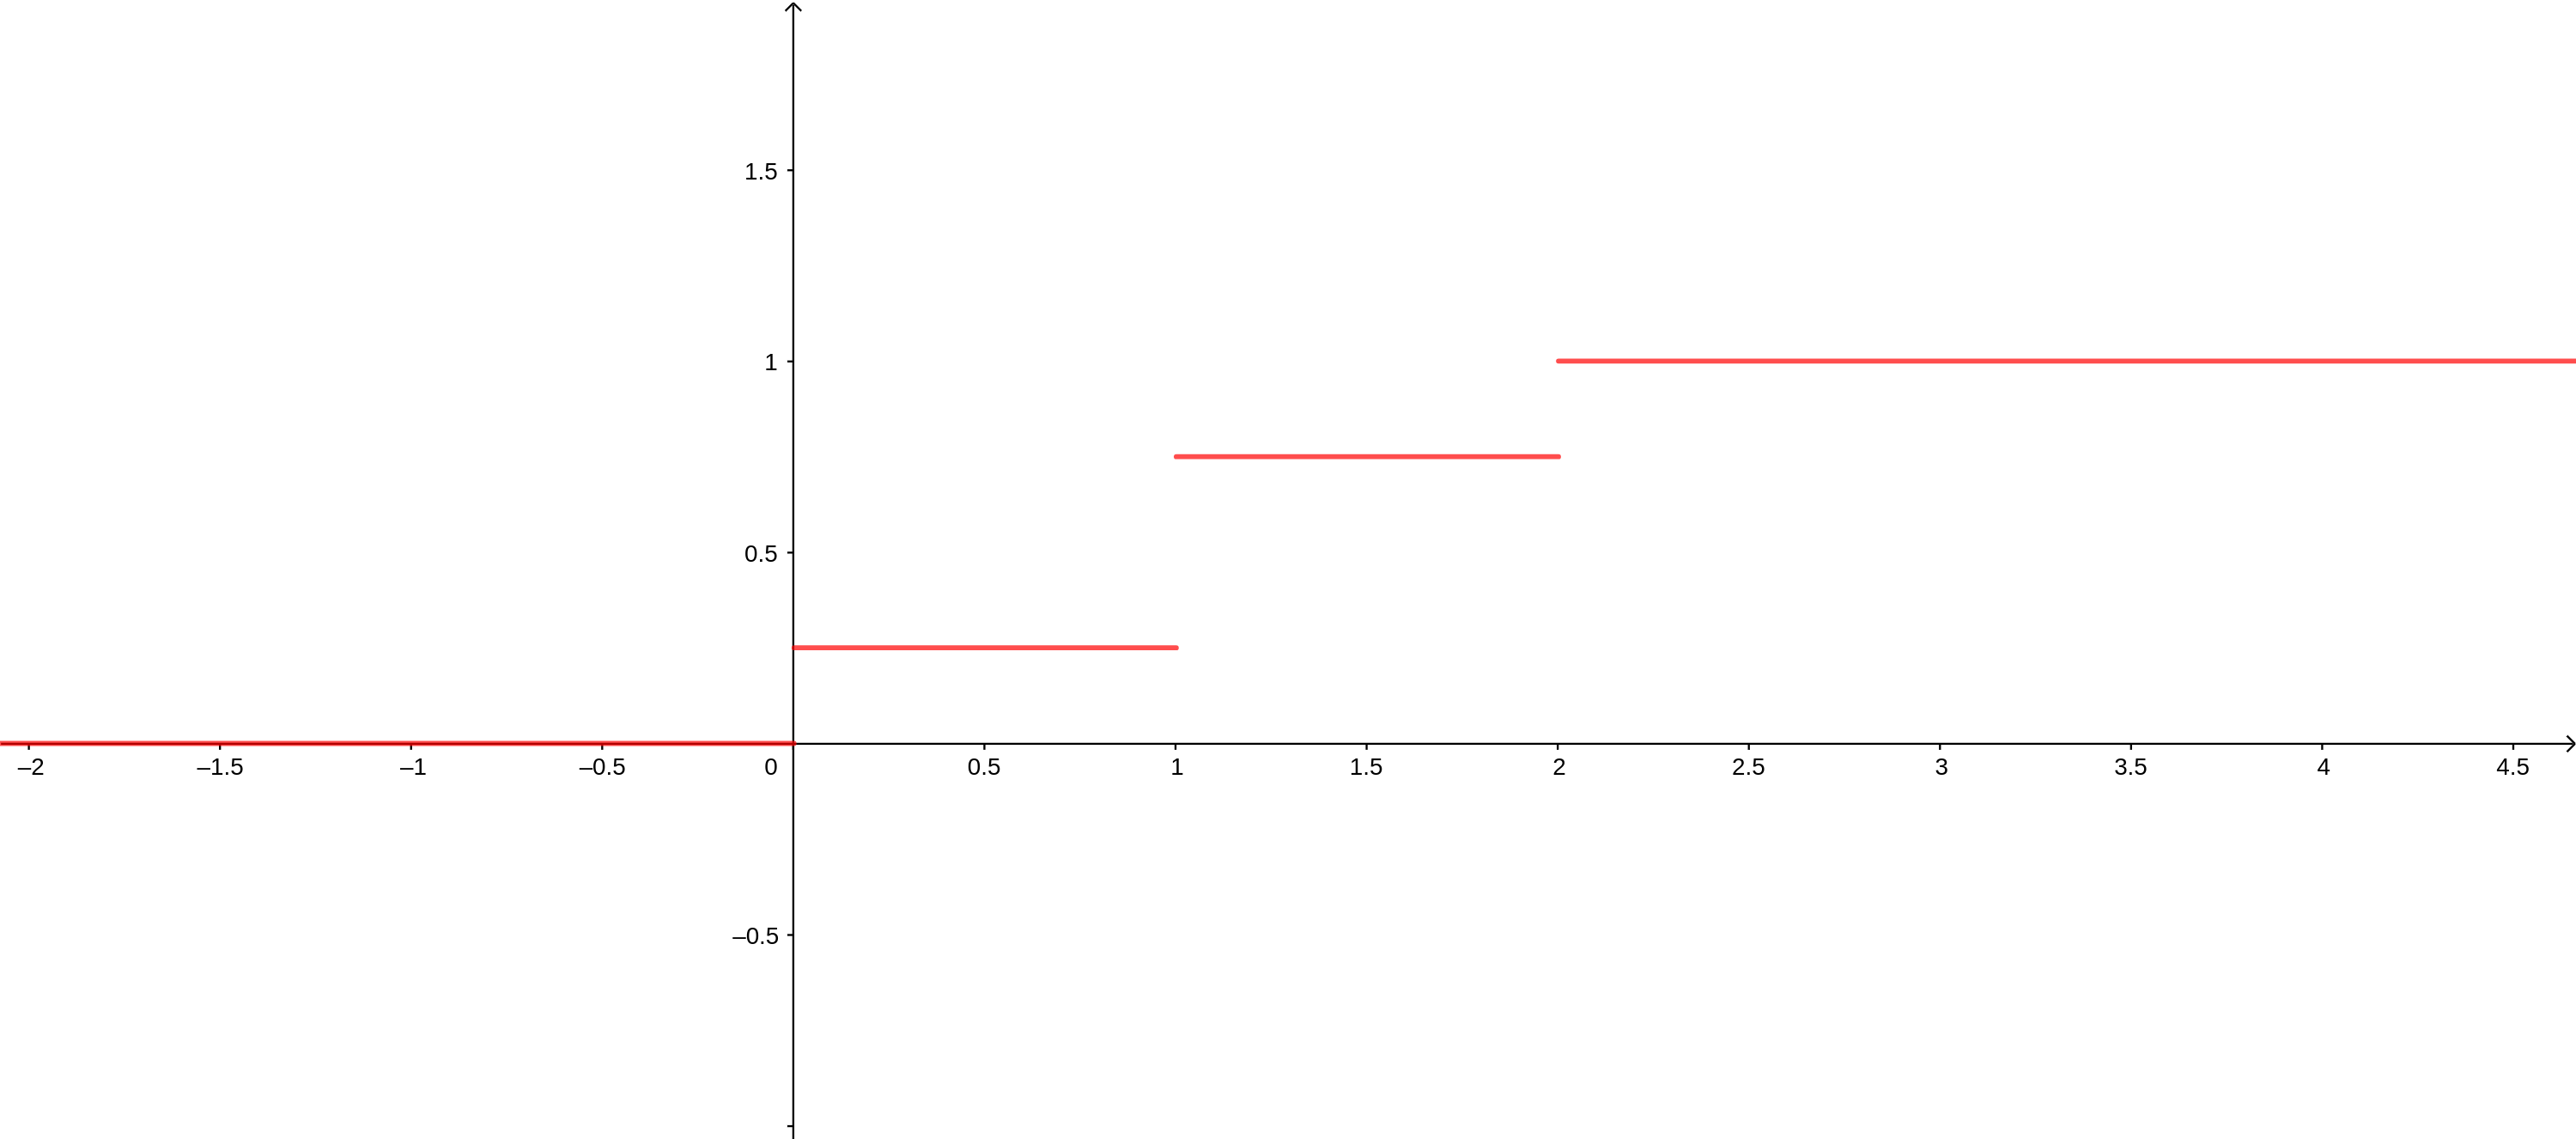
\includegraphics[width=\textwidth]{Imagens/fd1.png}
    \caption{Gráfico da f.d. anterior.}
%    \label{fig:my_label}
\end{figure}
\end{example}

\begin{example}
Sejam $(\Omega, \mathcal{A}, P)$ espaço de probabilidade, $c\in\mathbb{R}$ constante e $X$ v.a. em $(\Omega, \mathcal{A}, P)$ tal que $X(\omega) = c, \forall \omega\in\Omega$ (v.a. constante). Temos, então,
\begin{align*}
    p_X(x) &= \begin{cases}
    1, x = c \\
    0, \text{ c.c.}
    \end{cases} \\
    F_X(x) &= \begin{cases}
    0, x < c \\
    1, x\geq c
    \end{cases}
\end{align*}
\begin{figure}[H]
    \centering
    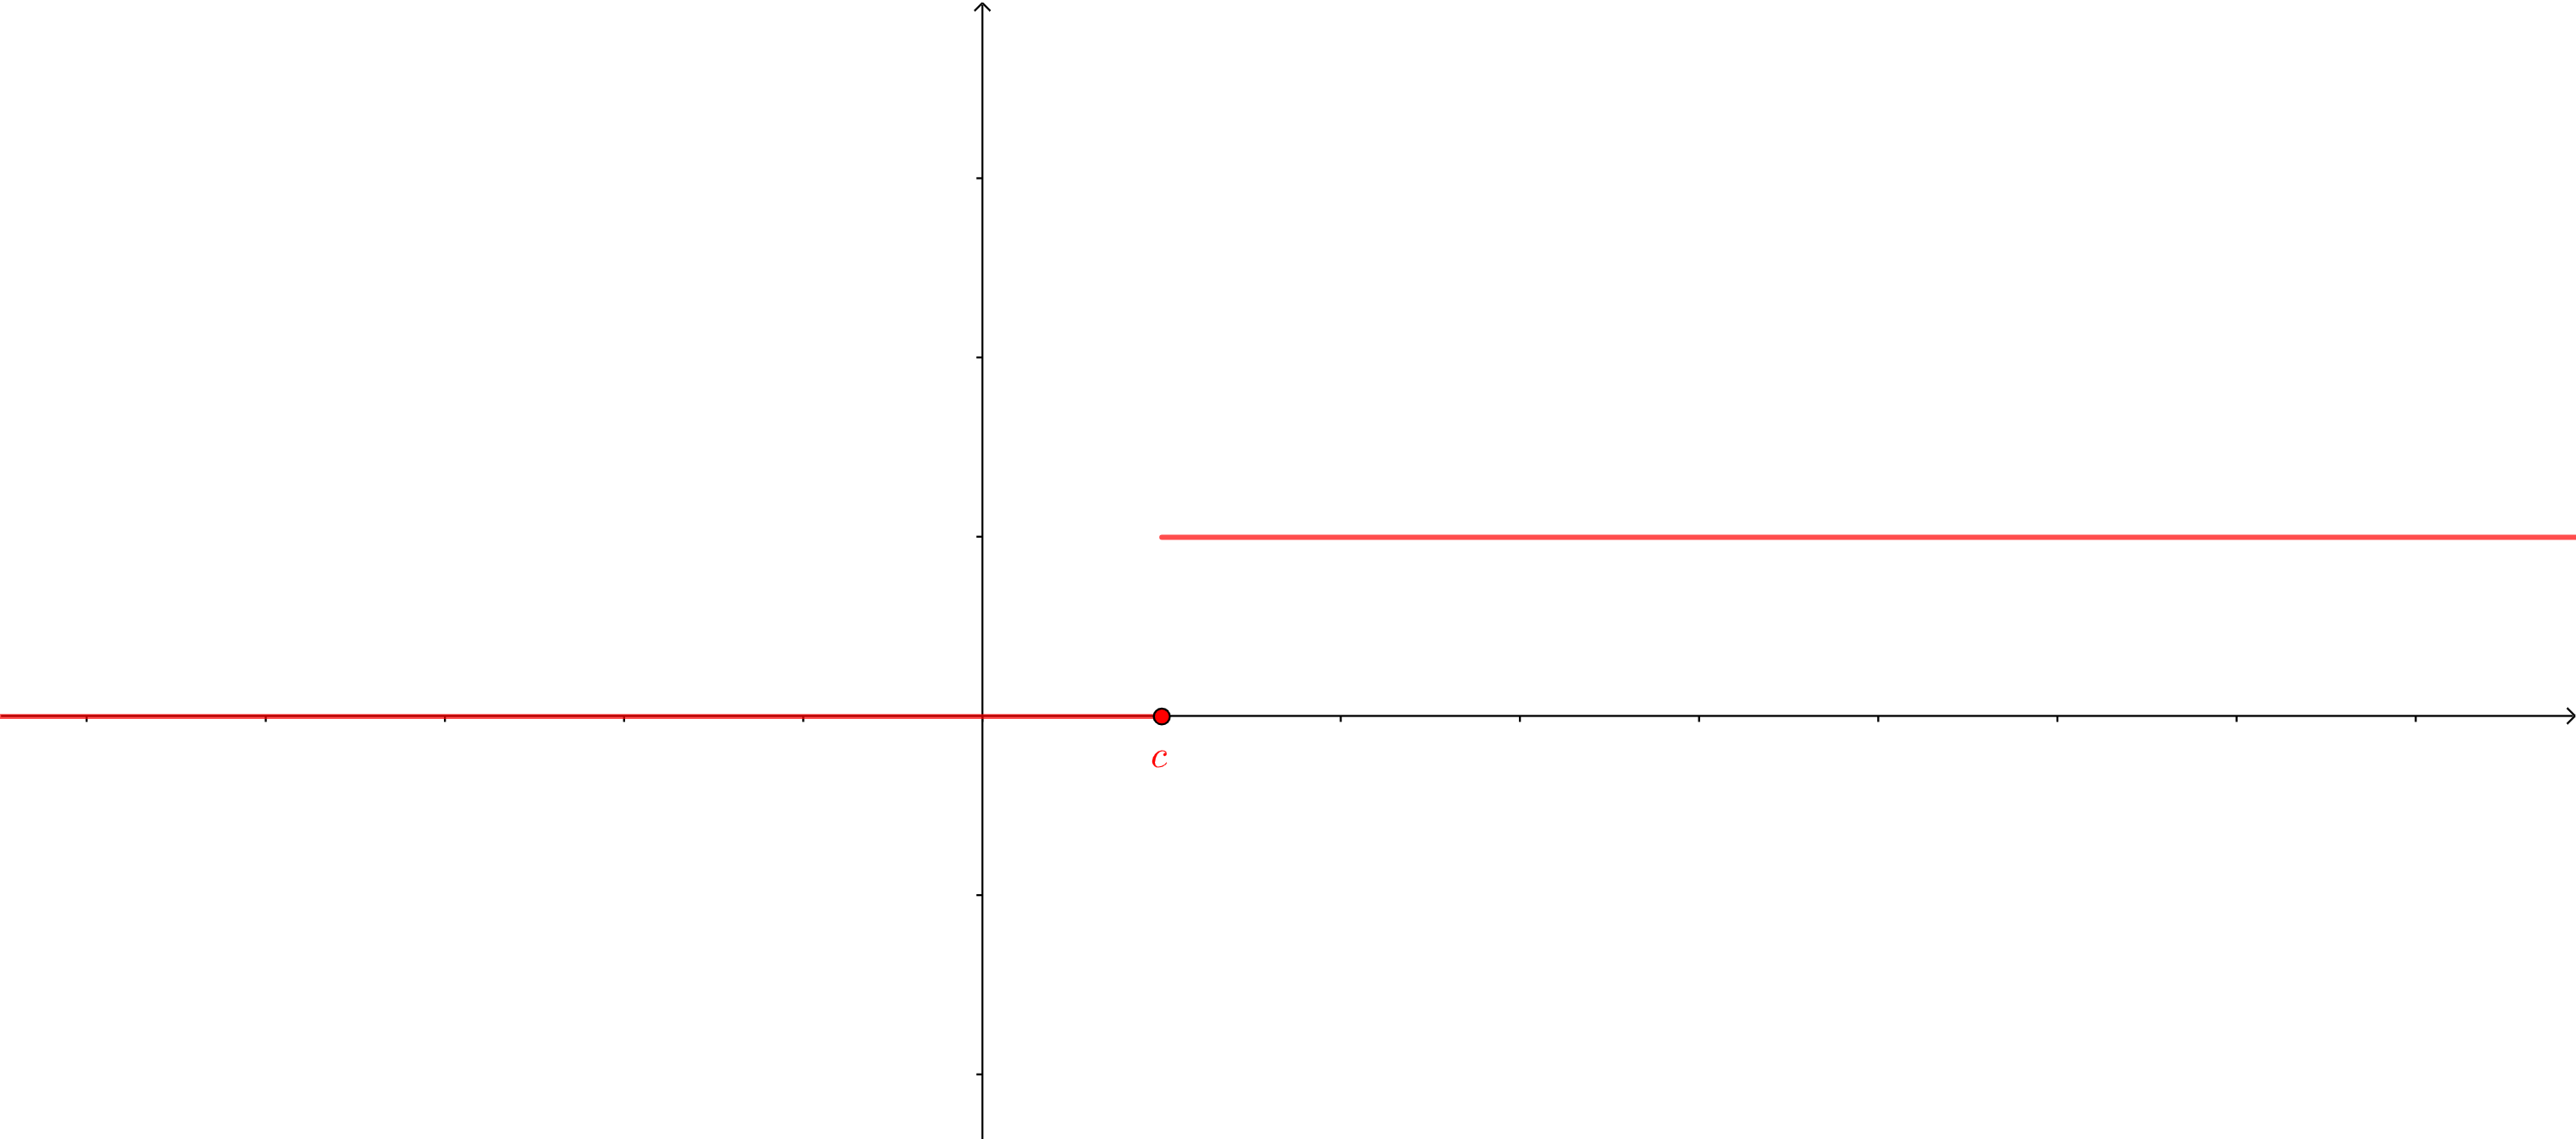
\includegraphics[width=\textwidth]{Imagens/fd2.png}
    \caption{Gráfico da f.d. anterior.}
%    \label{fig:my_label}
\end{figure}
\end{example}

\begin{example}
Seja $(\Omega, \mathcal{A}, P)$ espaço de probabilidade e $X\sim\text{Geom}(p), 0 < p < 1$. Temos
\begin{align*}
    p_X(k) = \begin{cases}
    p(1-p)^{k-1}, k = 1, 2, \dots \\
    0, \text{ c.c.}
    \end{cases}.
\end{align*}
Ademais, 
\begin{align*}
    \{X\leq x\} = \begin{cases}
    \emptyset, x\leq 1 \\
    \bigcup_{k=1}^{[x]} \{X=k\}, x\geq 1
    \end{cases}.
\end{align*}
Logo, como
\begin{align*}
    P\left( \bigcup_{k=1}^{[x]} \{X=k\} \right) = \sum_{k=1}^{[x]}P(X=k) = p\sum_{k=1}^{[x]}(1-p)^{k-1} = \frac{p}{1-p}\cdot (1-p)\frac{(1-(1-p)^{[x]})}{p} = 1 - (1-p)^{[x]},
\end{align*}
segue que
\begin{align*}
    F_X(x) = \begin{cases}
    0, x < 1 \\
    1 - (1-p)^{[x]}, x\geq 1.
    \end{cases}
\end{align*}
\end{example}

\begin{definition}[Perda de memória]
Uma v.a. $X$ é dita ter a propriedade de \textbf{perda de memória} se
\begin{enumerate}[(i)]
    \item $P(X>0)>0$;
    \item $P(X > a+b | X > a) = P(X>b), \forall a, b\geq 0$.
\end{enumerate}
\end{definition}

\begin{remark}
Note, em particular, que se $X$ é v.a. discreta com valores possíveis $1, 2, \dots$, então $X$ tem perda de memória se $P(X > n+m| X > n) = P(X>m), \forall n,m\in\{1, 2, \dots\}$. Ademais, se $X$ é v.a. qualquer, então dados $a,b\in\mathbb{R}_{>0}$ temos
\begin{align*}
    P(X > a+b | X > a) = P(X>b) \iff P(X>a+b) = P(X>a)P(X>b).
\end{align*}
\begin{proof}
De fato, 
\begin{align*}
    P(X > a+b| X>a) = P((X>a+b)\cap(X>a))/P(X>a) = P(X>a+b)/P(X>a).
\end{align*}
Logo,
\begin{align*}
    P(X > a+b | X>a) = P(X>b) \iff P(X>a+b) = P(X>a)P(X>b).
\end{align*}
\end{proof}
\end{remark}

\begin{proposition}
Seja $X$ v.a. discreta em $(\Omega, \mathcal{A}, P)$ assumindo valores em $\{1, 2, \dots\}$. Então $X$ tem perda de memória se, e só se, $X\sim\text{Geom}(p)$, para algum $0 < p < 1$.
\end{proposition}

\begin{proof}
($\Leftrightarrow$) Se $X\sim\text{Geom}(p), 0 < p < 1$, então
\begin{align*}
    P(X=k) = \begin{cases}
    p(1-p)^{k-1}, k = 1, 2, \dots \\
    0, \text{ c.c.}
    \end{cases}.
\end{align*}
Sejam $n,n\in\{1, 2, \dots\}$ quaisquer. Temos
\begin{align*}
    P(X > n+m | X > n) = \frac{P(X > n+m)}{P(X>n)} &= \sum_{k=0}^{\infty}p(1-p)^{n+m+k}/\sum_{k=0}^{\infty}p(1-p)^{n-k} \\
    &= \frac{ p(1-p)^{n+m}(1-(1-p))^{-1} }{ p(1-p)^n(1-(1-p))^{-1} } \\
    &= (1-p)^m \\
    &= P(X>m).
\end{align*}
($\Rightarrow$) Suponha que $X$ tenha perda de memória. Da proposição anterior, temos que
\begin{align*}
    P(X > n+m) = P(X>n)P(X>m), \forall n,m\in\{0,1,2,\dots\}.
\end{align*}
Se $n=0=m$, então
\begin{align*}
    P(X>0) = (P(X>0))^2 \Rightarrow P(X>0) = 0 \ \text{ ou } \ P(X>0) = 1.
\end{align*}
Como $X$ tem perda de memória, então $P(X>0) = 1$. Se $P(X=1) = p$, então $P(X>1) = 1 - p$. Daí, se $m\geq 1$, segue que
\begin{align*}
    P(X > m+1) = P(X>m)(1-p).
\end{align*}
Por indução, temos $P(X>m) = (1-p)^m, \forall m\in\{0, 1, 2, \dots\}$. Daí, dado $n\in\{1, 2, \dots\}$, temos
\begin{align*}
    P(X=n) = P(X>n-1) - P(X>n) = (1-p)^{n-1} - (1-p)^n = p(1-p)^{n-1},
\end{align*}
ou seja, $X\sim\text{Geom}(p)$.
\end{proof}

\begin{example}
Se $X\sim\text{Poisson}(\lambda)$, então
\begin{align*}
    p_X(k) = \begin{cases}
    e^{-\lambda}\frac{\lambda^k}{k!}, k = 0, 1, 2, \dots \\
    0, \text{ c.c.}
    \end{cases}
\end{align*}
e
\begin{align*}
    F_X(x) = \begin{cases}
    0, x < 0 \\
    e^{-\lambda}\sum_{k=0}^{[x]}\frac{\lambda^k}{k!}, x\geq 0
    \end{cases}.
\end{align*}
\end{example}

\begin{example}
Se $X\sim B(n,p)$, então
\begin{align*}
    p_X(k) = \begin{cases}
    \binom{n}{k}p^k(1-p)^{n-k}, k = 0, 1, \dots, n \\
    0, \text{ c.c.}
    \end{cases}
\end{align*}
e
\begin{align*}
    F_X(x) = \begin{cases}
    0, x<0 \\
    \sum_{k=0}^{[x]}\binom{n}{k}p^k(1-p)^{n-k}, x\geq 0
    \end{cases}.
\end{align*}
\end{example}

\begin{proposition}
Temos que a f.d. satisfaz as seguintes propriedades:
\begin{enumerate}[(i)]
    \item $0 \leq F_X(x) \leq 1, \forall x\in\mathbb{R}$;
    \item dados $x,y\in\mathbb{R}, x < y$, então $F_X(x)\leq F_X(y)$;
    \item $\forall a\in\mathbb{R}, F_X(a^+) := \displaystyle{\lim_{x\to a^+}F_X(x) = F_X(a)}$;
    \item $F_X(-\infty) := \displaystyle{\lim_{x\to -\infty}F_X(x) = 0}$ e $F_X(+\infty) := \displaystyle{\lim_{x\to +\infty}F_X(x) = 1}$.
\end{enumerate}
\end{proposition}

\begin{proof}
\begin{enumerate}[(i)]
    \item $F_X(x) = P(X\leq x) \Rightarrow 0\leq F_X(x) \leq 1, \forall x\in\mathbb{R}$.
    \item Dados $x,y\in\mathbb{R}, x<y,$ temos $\{X\leq x\} \subseteq \{X\leq y\}$ e, da monotonicidade da medida de probabilidade, $P(X\leq x)\leq P(X\leq y)$, i.e., $F_X(x)\leq F_X(y)$.
    \item Sejam $a\in\mathbb{R}$ e $(x_n)_{n\geq 1}$ uma sequência decrescente com $x_n \xrightarrow{n\to +\infty} a$. Temos $x_1\geq x_2\geq\cdots\geq a$, de modo que $\{X\leq x_1\}\supset\{X\leq x_2\}\supset\cdots$, ou seja, $(\{X\leq x_n\})_{n\geq 1}$ é uma sequência decrescente de eventos e
    \begin{align*}
        \lim_{n\to +\infty}\{X\leq x_n\} = \bigcap_{n=1}^{\infty}\{X\leq x_n\} = \{X\leq a\}.
    \end{align*}
    Pela continuidade da probabilidade, temos
    \begin{align*}
        F_X(a) = P(X\leq a) = \lim_{n\to +\infty}P(X\leq x_n) = \lim_{n\to +\infty} F_X(x_n) = \lim_{x\to a^+}F_X(x) := F_X(a^+).
    \end{align*}
    \item Seja $(x_n)_{n\geq 1}$ uma sequência decrescente tal que $x_n\xrightarrow{n\to +\infty} -\infty$. De $x_1\geq x_2\geq\cdots$, temos
    \begin{align*}
        \lim_{n\to +\infty}\{X\leq x_n\} = \bigcap_{n=1}^{\infty}\{X\leq x_n\} = \emptyset,
    \end{align*}
    donde
    \begin{align*}
        F_X(-\infty) := \lim_{x\to -\infty}F_X(x) = \lim_{n\to +\infty} F_X(x_n) = \lim_{n\to +\infty}P(X\leq x_n) = \lim_{n\to +\infty}P(\emptyset) = 0.
    \end{align*}
    Seja agora $(x_n)_{n\geq 1}$ crescente tal que $x_n\xrightarrow{n\to +\infty} +\infty$. De $x_1\leq x_2\leq\cdots$, temos $\{X\leq x_1\}\subset\{X\leq x_2\}\subset\cdots$, ou seja, 
    \begin{align*}
        \lim_{n\to +\infty}\{X\leq x_n\} = \bigcup_{n=1}^{\infty}\{X\leq x_n\} = \Omega.
    \end{align*}
    Logo, 
    \begin{align*}
        F_X(+\infty) := \lim_{x\to +\infty}F_X(x) = \lim_{x\to +\infty}P(X\leq x) = \lim_{n\to +\infty}P(X\leq x_n) = \lim_{n\to +\infty} P(\Omega) = 1.
    \end{align*}
\end{enumerate}
\end{proof}

\begin{remark}
Seja $X$ v.a. com f.d. $F_X$. A partir da f.d., podemos calcular $P(X\in A), \forall A\in\mathcal{B}(\mathbb{R})$:
\begin{enumerate}[(a)]
    \item se $A = (a,b]$, então $\{X\leq b\} = \{X\leq a\}\cup\{a<X\leq b\}$, donde
    \begin{align*}
        P(X\leq b) = P(X\leq a) + P(a < X\leq b),
    \end{align*}
    ou seja, 
    \begin{align*}
        P(X\in A) = P(a < X\leq b) = F_X(b) - F_X(a).
    \end{align*}
    \item se $A = (-\infty, b)$, temos $\{X\leq b\} = \displaystyle{\bigcup_{n=1}^{\infty}\{ X\leq b - 1/n \} }$, donde
    \begin{align*}
        P(X < b) = P\left( \bigcup_{n=1}^{\infty}\{ X\leq b - 1/n \} \right) &= \lim_{n\to +\infty} P(X\leq b - 1/n) \\
        &= \lim_{n\to +\infty}F_X(b - 1/n) \\
        &= \lim_{x\to b^-}F_X(x) := F_X(b^-).
    \end{align*}
    Logo, $P(X\in A) = P(X < b) = F_X(b^-) - \displaystyle{ \lim_{x\to b^-}F_X(x) }$.
    \item Se $A = \{a\}$, temos $\{ X\leq a \} = \{ X < a \}\cup\{X=a\}$, donde
    \begin{align*}
        P(X\leq a) = P(X<a)+P(X=a) \iff P(X=a) = F_X(a) - F_X(a^-).
    \end{align*}
    Raciocínios análogos valem para outros subintervalos da reta.
\end{enumerate}
Note também que como $F_X$ é contínua à direita e não decrescente, seus pontos de descontinuidade são do tipo salto, com tamanho $P(X=a) = F_X(a) - F_X(a^-)$ em $a$. Por fim, se $X$ é v.a. contínua, então $F_X$ é contínua.
\begin{proof}
De fato, dado $x\in\mathbb{R}$, temos
\begin{align*}
    0 = P(X=x) = F_X(x) - F_X(x^-),
\end{align*}
logo
\begin{align*}
    F_X(x) = F_X(x^-) = F_X(x^+), \forall x\in\mathbb{R}.
\end{align*}
\end{proof}
\end{remark}

\end{document}